\documentclass[../../main.tex]{subfiles}

\graphicspath{{../../image/}{../../figure/}}

\begin{document}

\section{自回归流}\label{section:ch18-自回归流}

我们注意到一组变量的联合分布总是可以写成条件分布的乘积，每个变量对应一个条件分布，由此可以推导出相关的标准化流公式（参见\cref{section:ch11-概率图模型}）。首先选择向量 $\bm{x}$ 中变量的顺序，我们可以在不失一般性的情况下写出：
\begin{align}
  p(x_1,\cdots,x_D)=\prod_{i=1}^{D}p(x_i\mid\bm{x}_{1:i-1}),\label{align:ch18-链式分解}
\end{align}
其中 $\bm{x}_{1:i-1}$ 表示 $(x_1,\cdots,x_{i-1})$。

\begin{proposition}[条件分布的链式分解]\label{proposition:ch18-链式分解}
设随机向量 $\bm{x}=(x_1,\cdots,x_D)$ 的联合密度为 $p$，且各条件密度 $p(x_i\mid\bm{x}_{1:i-1})$ 存在。则\eqref{align:ch18-链式分解}成立；特别地，当 $i=1$ 时约定 $\bm{x}_{1:0}$ 为空，$p(x_1\mid\bm{x}_{1:0})=p(x_1)$。
\end{proposition}

\begin{proof}（重构新增）
对 $D$ 归纳。$D=1$ 时\eqref{align:ch18-链式分解}两端都是 $p(x_1)$，按空条件的约定成立。

设结论对 $D-1$ 成立。由条件密度的定义（见\cref{section:ch02-概率密度}），在 $p(x_1,\cdots,x_{D-1})>0$ 的点处有
\begin{align*}
  p(x_1,\cdots,x_D)=p(x_D\mid\bm{x}_{1:D-1})\,p(x_1,\cdots,x_{D-1}).
\end{align*}
右端第二个因子由归纳假设等于 $\prod_{i=1}^{D-1}p(x_i\mid\bm{x}_{1:i-1})$，代入即得\eqref{align:ch18-链式分解}。若某点处 $p(x_1,\cdots,x_{D-1})=0$，则左端也为零，等式仍成立。
\end{proof}

% SUPPLEMENT: parent=proposition:ch18-链式分解; kind=motivation; location=紧随其后的 remark（重构新增）
\begin{remark}（重构新增）
这个恒等式本身只是概率的乘积法则反复使用，但它是自回归建模的全部起点：它把一个 $D$ 维联合分布的问题拆成 $D$ 个一维条件分布的问题，而每个一维条件分布都可以用一个神经网络来参数化（例如取成均值和方差由网络给出的 Gauss 分布）。\cref{section:ch11-序列模型}中的自回归模型正是按这个思路构造的。

条件方面：结论只要求各条件密度存在，对变量是离散还是连续、条件依赖哪一段前缀都没有限制。所谓“不失一般性”指的是变量的排列顺序可以任意选定：换一个顺序就换一种分解，\eqref{align:ch18-链式分解}对任何顺序都成立，但不同的顺序给出不同的模型族（这与\cref{chapter:ch11-结构化分布}中讨论的变量顺序问题同源）。

与标准化流的联系在于：若把每个条件分布的实现写成 $x_i=h(z_i,g_i(\bm{x}_{1:i-1}))$，其中 $z_i$ 取自简单的基础分布，那么整条变换的 Jacobian 自动是三角的——因为 $x_i$ 只依赖 $\bm{x}_{1:i-1}$ 与 $z_i$，不依赖 $z_{i+1},\cdots,z_D$。三角结构又让行列式变成对角元之积，于是似然可以精确而廉价地计算。这正是下面两个模型的共同机制。
\end{remark}

这种因式分解可以用来构建一类称为\textbf{掩码自回归流}（Masked Autoregressive Flow, MAF）（Papamakarios, Pavlakou, and Murray, 2017）的标准化流，如下所示：

\begin{definition}[掩码自回归流]\label{definition:ch18-掩码自回归流}
设潜变量为 $\bm{z}=(z_1,\cdots,z_D)$、数据变量为 $\bm{x}=(x_1,\cdots,x_D)$。掩码自回归流是形如
\begin{align}
  x_i=h\big(z_i,g_i(\bm{x}_{1:i-1},\bm{w}_i)\big)\label{align:ch18-maf}
\end{align}
的变换，其中 $h(z_i,\cdot)$ 是耦合函数，因为对每个给定的条件值都可以很容易地对 $z_i$ 求逆；$g_i$ 是条件函数，通常用一个深度神经网络来表示，$\bm{w}_i$ 是它的参数。
\end{definition}

% SUPPLEMENT: parent=definition:ch18-掩码自回归流; kind=motivation; location=紧随其后的 remark（重构新增）
\begin{remark}（重构新增）
动机：\eqref{align:ch18-链式分解}把联合密度拆成条件密度之积，而\eqref{align:ch18-maf}正是“逐坐标地把基础分布的条件分位数搬运成数据的条件分布”的实现。因为第 $i$ 个输出只用到前 $i-1$ 个输入，整条变换天然是三角的，于是既能精确算似然，又能保持可逆。

条件方面：$h(z_i,\cdot)$ 只需在“第一个变量”方向上可逆，对条件函数 $g_i$ 没有任何可逆性要求（这与耦合流中的技巧完全相同）；$\bm{w}_i$ 允许随 $i$ 不同，实际实现中常让所有 $i$ 共享一个网络、靠掩码区分。

一个容易忽略的细节：\eqref{align:ch18-maf}要求 $x_i$ 只依赖 $\bm{x}_{1:i-1}$ 而不依赖 $\bm{x}_{i+1:D}$，这正是“自回归”的含义，也是三角性的来源。若破坏了这一依赖结构，行列式就不再是三角的，计算代价立刻回到 $\mathcal{O}(D^{3})$。
\end{remark}

\cref{figure:ch18-自回归流结构}(a) 说明了这一点。术语“掩码”指的是使用单个神经网络来实现一组形式为\eqref{align:ch18-maf}的方程，连同一个二进制掩码（Germain et al., 2015）来强制网络权重的一个子集为零，以实现自回归约束［\eqref{align:ch18-链式分解}］。

在这种情况下，计算似然函数所需的逆运算如下：

\begin{proposition}[掩码自回归流的逆与三角 Jacobian]\label{proposition:ch18-maf逆}
设掩码自回归流由\eqref{align:ch18-maf}给出，且每个 $h(z_i,\cdot)$ 对固定的条件值都是 $z_i$ 的可逆函数。则计算似然函数所需的逆运算为
\begin{align}
  z_i=h^{-1}\big(x_i,g_i(\bm{x}_{1:i-1},\bm{w}_i)\big).\label{align:ch18-maf逆}
\end{align}
由于\eqref{align:ch18-maf逆}中 $z_1,\cdots,z_D$ 这些分项函数只依赖已知的 $\bm{x}$，它们可以并行计算，因此评估以上似然函数的操作在现代硬件上就能高效执行。对应于这组变换的 Jacobian 矩阵的元素为 $\partial z_i/\partial x_j$，这些元素形成一个三角矩阵，其行列式由对角线元素的乘积给出，因此也可以高效计算（见\cref{exercise:ch18-04}）。
\end{proposition}

\begin{proof}（重构新增）
先证\eqref{align:ch18-maf逆}。由\eqref{align:ch18-maf}，$x_i=h\big(z_i,g_i(\bm{x}_{1:i-1},\bm{w}_i)\big)$，其中条件值 $g_i(\bm{x}_{1:i-1},\bm{w}_i)$ 只依赖 $\bm{x}$ 的前 $i-1$ 个分量、与 $z_i$ 无关。对固定的条件值把 $h(\cdot,g_i)$ 反解，即得\eqref{align:ch18-maf逆}；由于每个 $z_i$ 的右端只用到已知的 $\bm{x}$，这 $D$ 个式子之间没有依赖，可以并行求值。

再证三角性。由\eqref{align:ch18-maf逆}，$z_i$ 只依赖 $x_1,\cdots,x_i$，与 $x_{i+1},\cdots,x_D$ 无关，故当 $j>i$ 时
\begin{align*}
  \frac{\partial z_i}{\partial x_j}=0,
\end{align*}
即 $\bm{J}$ 的主对角线以上元素全为零，它是下三角矩阵。下三角矩阵的行列式等于对角元之积，
\begin{align*}
  \det\bm{J}=\prod_{i=1}^{D}\frac{\partial z_i}{\partial x_i},
\end{align*}
其中 $\partial z_i/\partial x_i=\partial h^{-1}(x_i,g_i)/\partial x_i$（固定条件值求导），于是只需 $D$ 次一维求导即可得到行列式。
\end{proof}

% SUPPLEMENT: parent=proposition:ch18-maf逆; kind=motivation; location=紧随其后的 remark（重构新增）
\begin{remark}（重构新增）
这条结论说明掩码自回归流在“评估似然”这一方向上极其高效：一次前向就能得到全部 $z_i$，行列式只是 $D$ 个对角元的乘积，总代价与一次普通网络前向同阶。代价出在反方向上：要从 $\bm{z}$ 生成 $\bm{x}$，必须按 $i=1,2,\cdots,D$ 的顺序逐个计算 $x_i$（因为 $x_i$ 依赖 $\bm{x}_{1:i-1}$），无法并行，见本节末的比较。

条件方面：结论只用到“$h$ 对第一个变量可逆”这一条，以及\eqref{align:ch18-maf}的依赖结构；对 $g_i$ 没有额外要求。若 $h$ 不是逐元素的，而是把 $z_i$ 与条件值混合的一般可逆函数，只要它仍只依赖 $\bm{x}_{1:i-1}$，三角性与行列式结论都不变。

\textbf{原文问题说明。} 正文此处印作“这些元素形成一个上三角矩阵”，这与\cref{exercise:ch18-04}的说法（“下三角矩阵”）以及\eqref{align:ch18-Jacobian元素}的约定 $J_{ij}=\partial z_i/\partial x_j$ 都不一致：按该约定，$j>i$ 时元素为零，得到的是下三角矩阵；只有在把矩阵转置（即用 $J_{ij}=\partial z_j/\partial x_i$ 排布）时它才表现为上三角。两种写法不影响“行列式等于对角元之积”这一实质结论，也不影响计算代价，但读者应以\cref{exercise:ch18-04}的“下三角”为准。
\end{remark}

然而，从该模型中抽样的任务必须通过计算\eqref{align:ch18-maf}来完成，这本质上是一个顺序执行的过程，因为在计算 $x_i$ 之前必须先计算 $x_1,\cdots,x_{i-1}$ 的值，所以速度较慢。为了避免这种效率低下的抽样，我们可以定义\textbf{逆自回归流}（Inverse Autoregressive Flow, IAF）（Kingma et al., 2016），如下所示：

\begin{definition}[逆自回归流]\label{definition:ch18-逆自回归流}
逆自回归流是形如
\begin{align}
  x_i=h\big(z_i,\tilde{g}_i(\bm{z}_{1:i-1},\bm{w}_i)\big)\label{align:ch18-iaf}
\end{align}
的变换，其中 $\tilde{g}_i$ 是条件函数，$h(z_i,\cdot)$ 是耦合函数。它与\eqref{align:ch18-maf}的唯一差别在于：条件函数依赖的是潜变量的前缀 $\bm{z}_{1:i-1}$，而不是数据变量的前缀 $\bm{x}_{1:i-1}$。
\end{definition}

% SUPPLEMENT: parent=definition:ch18-逆自回归流; kind=motivation; location=紧随其后的 remark（重构新增）
\begin{remark}（重构新增）
把条件函数的输入从 $\bm{x}_{1:i-1}$ 换成 $\bm{z}_{1:i-1}$，看似只是记号上的小改动，实际上交换了“便宜的方向”：\eqref{align:ch18-iaf}的右端只用到 $\bm{z}$，所以给定 $\bm{z}$ 时所有 $x_i$ 可以一次算出；而似然方向必须反解\eqref{align:ch18-iaf}，反解 $z_i$ 需要 $\tilde{g}_i(\bm{z}_{1:i-1},\bm{w}_i)$，后者又依赖尚未求出的 $z_1,\cdots,z_{i-1}$，于是只能顺序进行。

条件方面：与掩码自回归流相同，只要求 $h(\cdot,g)$ 可逆；$\tilde{g}_i$ 可以是任意网络。注意 $\tilde{g}$ 上的波浪号只是为了与\eqref{align:ch18-maf}中的 $g$ 区分，两者在结构上没有本质不同。

这个定义也解释了为什么两种流要做成“对偶”的样子：可逆变换的两个方向（采样、求似然）中总有一个是顺序的，除非像耦合流那样把坐标分成两组。这种“一个方向快、另一个方向慢”的取舍无法同时消除，只能依应用选择。
\end{remark}

如\cref{figure:ch18-自回归流结构}(b) 所示，对于给定的 $\bm{z}$，可以使用\eqref{align:ch18-iaf}并行计算元素 $x_1,\cdots,x_{i-1}$，因此采样效率提高了。然而，计算似然所需的逆函数需要一系列如下形式的计算：

\begin{proposition}[逆自回归流的逆]\label{proposition:ch18-iaf逆}
设逆自回归流由\eqref{align:ch18-iaf}给出，且每个 $h(z_i,\cdot)$ 对固定的条件值都是 $z_i$ 的可逆函数。则似然方向所需的计算为
\begin{align}
  z_i=h^{-1}\big(x_i,\tilde{g}_i(\bm{z}_{1:i-1},\bm{w}_i)\big),\label{align:ch18-iaf逆}
\end{align}
这些计算本质上是顺序进行的：$z_i$ 的右端依赖 $z_1,\cdots,z_{i-1}$，必须逐个求解；而采样方向给定 $\bm{z}$ 后可以并行。
\end{proposition}

\begin{proof}（重构新增）
\eqref{align:ch18-iaf逆}由\eqref{align:ch18-iaf}对第一个变量反解得到，因为 $\tilde{g}_i(\bm{z}_{1:i-1},\bm{w}_i)$ 与 $z_i$ 无关。顺序性来自右端的依赖：要算 $z_i$ 必须先知道 $z_1,\cdots,z_{i-1}$，故 $z_1$ 先算，之后 $z_2$，依此类推，共 $D$ 步串行，不能并行。

反过来，给定 $\bm{z}$ 后，\eqref{align:ch18-iaf}的右端对每个 $i$ 只用到已知的 $\bm{z}_{1:i-1}$，$D$ 个式子互不依赖，可以一次并行算出全部 $x_i$。
\end{proof}

% SUPPLEMENT: parent=proposition:ch18-iaf逆; kind=motivation; location=紧随其后的 remark（重构新增）
\begin{remark}（重构新增）
把这条与\cref{proposition:ch18-maf逆}并排看，就得到自回归流的“对偶表”：掩码自回归流评估似然是 $\mathcal{O}(1)$ 次并行前向、采样是 $D$ 步串行；逆自回归流恰好相反。两者都需要 $D$ 步串行完成其中一个方向，因此当 $D$ 很大（例如高分辨率图像）时，串行的一侧会成为瓶颈。

条件方面：两条命题的前提完全相同（$h$ 对第一个变量可逆），差别只在条件函数的输入。

\textbf{原文问题说明。} 正文把可并行计算的元素写作 $x_1,\cdots,x_{i-1}$，按上下文应为 $x_1,\cdots,x_D$：给定 $\bm{z}$ 后，\eqref{align:ch18-iaf}右端对每个 $i$ 都只用到已知的 $\bm{z}_{1:i-1}$，因此全部 $x_i$ 都可一次并行算出，而不只是前 $i-1$ 个。这不影响“逆自回归流采样快、似然慢”的结论。
\end{remark}

\begin{figure}[htbp]
  \centering
  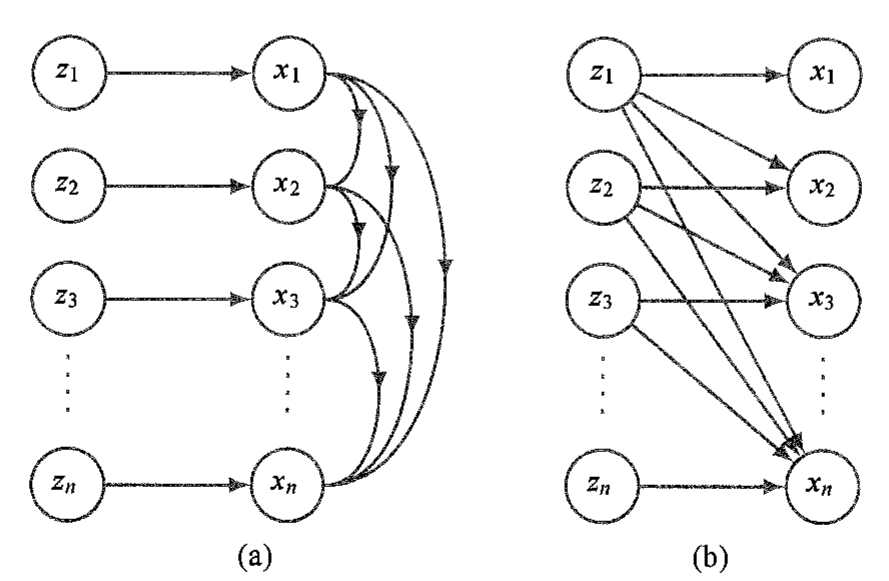
\includegraphics[width=0.75\textwidth]{ch18-fig501-ar-flows.png}
  \caption{两种自回归标准化流的结构示意图。(a) 中显示的掩码自回归流允许对似然函数进行有效评估，而 (b) 中显示的替代逆自回归流允许进行高效抽样}
  \label{figure:ch18-自回归流结构}
\end{figure}

这些计算本质上是顺序进行的，因此速度很慢。具体应该使用掩码自回归流还是逆自回归流取决于特定的应用。

耦合流和自回归流是密切相关的。尽管自回归流引入了相当大的灵活性，但由于需要顺序地依次采样，这带来了随数据空间维数 $D$ 线性增长的计算成本。耦合流可以视为自回归流的一个特例，它将变量分成两组而不是 $D$ 组，提升了效率，但牺牲了一些通用性。

\end{document}
